
\chapter[Revisão Teórica]{Revisão Teórica}
  Esse capítulo irá apresentar alguns conceitos que irão sustentar o objetivo deste trabalho.
Desse modo este capítulo está dividido nas seções: Importância da análise do movimento humano (\ref{sec:importancia}),
Engenharia de Software (\ref{sec:engenhariaSoft}), Aquisição de dados com Sensores (\ref{sec:aquisicaoSensores}),
Processamento de sinais (\ref{sec:processamentoSinais}), Articulações no corpo humano (\ref{sec:Juntas no corpo humano}), Restrição - Tempo real (\ref{sec:restrição}),
Trabalho relacionado (\ref{Sec:MetCondTCC}), Requisitos (\ref{Sec:Requisitos}) e Arquitetura de software (\ref{Sec:arquitetura}).

\section{Importância da análise do movimento humano}\label{sec:importancia}

A mensuração do movimento humano é uma forma de observação, através da utilização
de dispositivos, para descrever os fenômenos em termos de variáveis a serem analisadas.
Os dados adquiridos a partir da mensuração podem elucidar deficiências
motoras após trauma ou esclarecer os efeitos de intervenção externa controlada.
Eles são usados para descrever, caracterizar, medir o impacto dos
fatores externos e analisar o movimento humano. Dados cinemáticos e cinéticos podem ser combinados
e analisados para explicar as características do movimento.

Além da qualidade das medições, tem-se que considerar a complexidade da medição
feita por determinado dispositivo, tais como a necessidade do paciente se despir,
necessidade de uma grande área para a medição, entre outros.

Em estudos do movimento humano, existem essencialmente três tipos de variáveis de medição: tempo,
cinemática e cinética. O tempo pode ser utilizado isoladamente para medir a duração de um determinado movimento
, mas fornece mais informações quando associado a uma variável cinemática ou cinética.
As variáveis cinemáticas descrevem o movimento do corpo, que são lineares (deslocamento,
velocidade e aceleração) ou angular (deslocamento, velocidade e aceleração).
 As variáveis cinéticas são ou o momento de força ou força que gera o movimento \cite{roberto}.

A análise do movimento humano é imprescindível não somente para a avaliação e a
reabilitação do indivíduo, mas também para prevenção de lesões. Vale ressaltar que
lesões recorrentes em esportistas é extremamente prejudicial não somente a sua saúde
mas também ao seu desempenho no esporte influenciando diretamente ao seu retorno a
prática do mesmo. A Biomecânica  permite analisar as causas e efeitos
produzidos em relação a otimização do rendimento do atleta, o comportamento da
sobrecarga articular e os efeitos dos mecanismos motores no processo de aprendizagem
são fatores, que se relacionam com o diagnóstico da técnica esportiva, e o trabalho
preventivo principalmente em atletas de alto rendimento. Para a investigação deste
movimento, torna-se necessário, pela complexidade estrutural do mesmo, a aplicação
simultânea de métodos de mensuração nas diversas áreas do conhecimento da ciência. O
estudo do movimento permite-nos verificar, avaliar, reabilitar e prevenir por exemplo:
  \begin{enumerate}
  \item Esporte de alto nível de rendimento: sistematização e otimização do rendimento
  esportivo, diagnostico da técnica de movimento e condição física, redução de
  sobrecargas excessivas ao aparelho locomotor, regime de treinamento preventivo e que
  maximize o desempenho do atleta e relação estímulo-resposta;
  \item Esporte escolar, de baixo rendimento e atividades de recreação/musculação: estudo
  da eficiência de processos de aprendizagem, adequação de sistemas e equipamentos
  com “feedback” pedagógico; otimização de desempenho em pratica esportiva;
  prevenção de lesões em atletas que reproduzem movimentos repetitivos; indivíduos
  saudáveis com o objetivo de hipertrofia;
  \item Prevenção e reabilitação orientados à saúde: desenvolvimento de métodos,
  procedimentos e técnicas aplicados à terapia, descrição de padrões “patológicos” e
  dependências clinicas, adequação e desenvolvimento de equipamentos;
  \item Atividades do cotidiano e do trabalho: estudo da postura e da locomoção humana,
  classificação e sistematização de grupos de movimentos em dependência de estações de
  trabalho, interface homem, máquina e meio ambiente, eficiência, saúde e segurança nas
  tarefas da vida diária e do trabalho \cite{contextBiomecanica}.
  \end{enumerate}

\subsection{Análise de dados cinéticos e cinemáticos}
Quando os dados de cinemática ou cinética é indexado com o tempo, o resultado é uma série temporal cinemático
 ou cinético. A ferramenta mais comum para analisar essas séries temporais são os
gráficos resultantes, pois é mais fácil visualizar o padrão de movimento. A inclinação e
curvatura do gráfico de séries temporais indicam características-chave de uma
 execução do movimento e fornece uma poderosa ferramenta para análise de movimento.
A Figura \ref{sentar-para-levantar-para-sentar} tirada do trabalho do Baptista \cite{roberto},mostra o deslocamento angular do
joelho e do tronco durante um ciclo de marcha sentar-para-levantar-para-sentar. Analisando as encostas e pontos de inflexão, é
possível determinar o início e o fim de cada flexão ou extensão para esta determinada
articulação.

Partindo da premissa de que o mesmo movimento executado por diferentes indivíduos irão
ter um padrão semelhante, as medições de séries temporais de dados cinemáticos e
 cinéticos podem ser anotados para a extração de informações de
desempenho quantitativo. Exemplo de tais análises pode ser encontrado em diagramas de ciclo de marcha, que são os mais comuns.

A análise da marcha é um campo bem estabelecido de estudo, principalmente devido
ao uso do diagrama de ciclo de marcha, como uma ferramenta para descrever,
relatar e comparar o desempenho da marcha em diferentes resultados da investigação.
Devido ao sucesso do diagrama de ciclo de marcha, os investigadores propuseram igualmente descrições padronizadas para
outros tipos de movimento, tais como o movimento senta-levanta-senta e também atividades esportivas.

A Figura \ref{sentar-para-levantar-para-sentar} mostra os diagramas de ciclo de movimento para a marcha e sentar-para-levantar-para-sentar .

\begin{figure}[H]
\centering
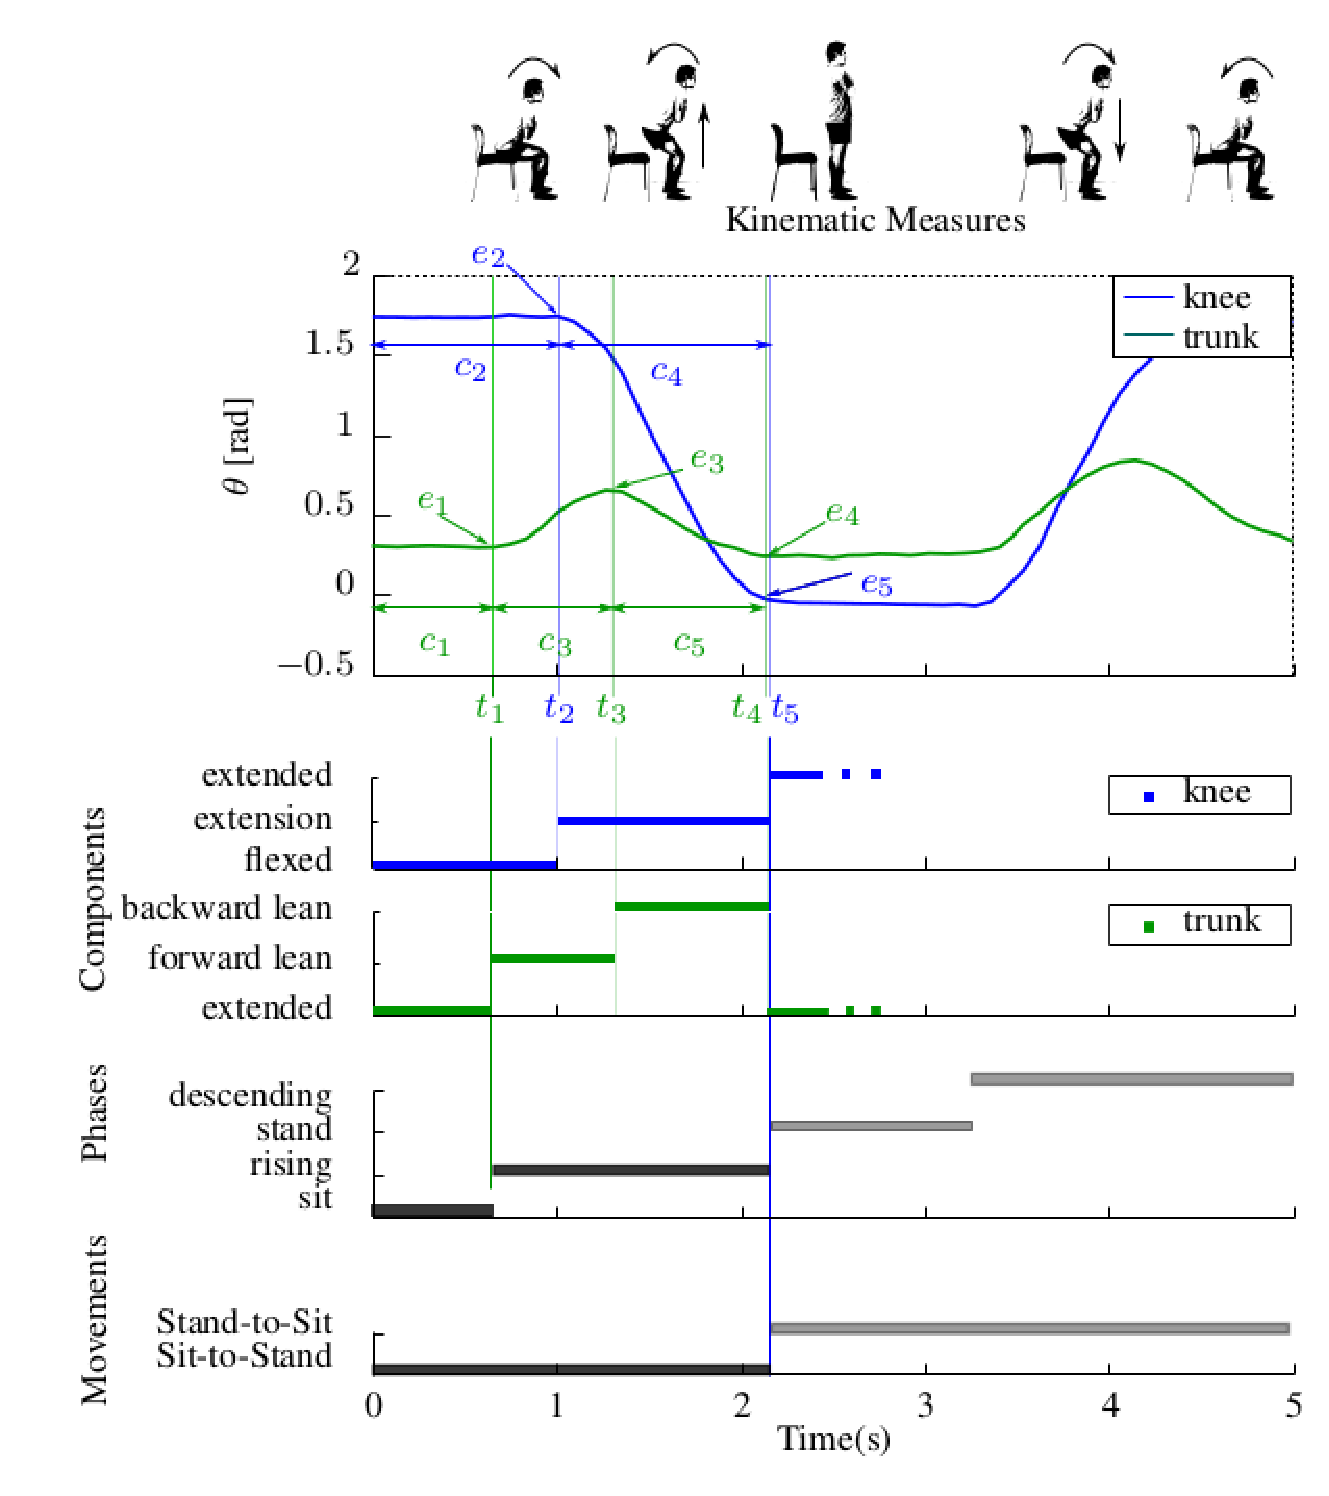
\includegraphics [keepaspectratio=true,scale=0.60]{figuras/sentaLevanta.eps}
\caption{Sentar-para-levantar-para-sentar. Fonte: \cite{roberto}.}

\label{sentar-para-levantar-para-sentar}
\end{figure}

\subsection{Automatizando a análise do movimento}
  É muito comum sistemas de análise automático de movimento.
Um exemplo disso é o kinect da microsoft que se encaixa como sendo de baixo custo, que
extrai as coordenadas das articulações nos usuários e são usados como sinal de entrada de jogos e aplicativos.
Além do Kinect, outros sensores são disponíveis no mercado para obtenção de precisão de dados da cinemática humana, fazendo com que essa informação seja hoje acessível e disseminado.
Porém, as técnicas de pós-processamento para extração de recurso automático de dados cinemáticos ainda estão surgindo.

Uma vez extraído dados das articulações no decorrer do tempo, esses dados devem ser identificados para segmentar/classificar movimentos pré-definidos.
  No contexto da segmentação do movimento humano e classificação para a reabilitação,
uma importante distinção deve ser feita sobre o significado da tarefa de segmentação e classificação.
Um problema é segmentar uma sequência de movimentos desconhecidos e
individuais, seguidos pela classificação do tipo de movimento (rotulando cada única
 execução de acordo com um conjunto de possíveis candidatos).
Este problema foi recentemente investigada com resultados importantes, tais como
feito por \cite{LinaAndDkulic} e \cite{PdeDios}. Outro problema é: dada uma única
execução (ou uma sequência repetitiva) de um tipo conhecido do movimento
 (uma sequência de passos, ou uma sequência de senta-levanta-senta), identificar os principais eventos,
a fim de extrair informações úteis, ou seja, características espaço-temporais \cite{roberto}.

O trabalho apresentando em \cite{roberto} investiga técnicas para análise automática
do movimento humano. Sua principal contribuição é um novo procedimento para avaliação
automática do movimento humano que executa segmentação e extração de parâmetros de
desempenho motor em séries temporais de medidas de uma sequência de movimentos. Nele,
utiliza os elementos de um modelo de Sistema Linear Dinâmico Chaveado como componentes
 de base para traduzir definições formais e procedimentos utilizados na análise de
movimento tradicional. Sua abordagem estabelece um método que permite usuários sem
experiência em processamentos de sinais criarem modelos para movimentos a partir de dados rotulados e usá-los posteriormente para avaliação automática. No trabalho é validado o
procedimento com conjunto de dados coletados de seis indivíduos sadios que executaram
movimentos comuns em testes funcionais e sessões de exercícios de reabilitação, tais como
o sentar-e-levantar e elevação lateral dos braços.

Existe três estágios para utilização do sistema. Primeiro uma pessoa qualificada
executa um exercício ou uma sessão de exercício que é armazenado. Neste estágio,
o Kinect é controlado através de uma função matlab, que foi escolhido por ser otimizado para resolução de problemas científicos e de engenharia e onde
 a linguagem MATLAB é a maneira mais natural do mundo para expressar matemática computacional \cite{matlab}, e é especificamente desenvolvida
para GUI (\textit{Graphic User interface} - Interface gráfica do usuário). Esta
função baseia-se em tarefas periódicas para captar e armazenar os pontos 3D, bem
como as imagens capturadas pelo Kinect. Os pontos 3D compõem a representação de
um esqueleto do usuário, que estão em referência a posição do Kinect. Estes pontos
são obtidos utilizando a função NITE \cite{openNI} chamado pelo Matlab via C++
wrapper. Até o fim da captura, os dados dos pontos são armazenados em um arquivo
.mat e disponível para uma visualização posterior.

No segundo estágio, o usuário pode ver a reprodução do movimento previamente armazenado
antes de começar a sessão. Isso é feito em Matlab com funções especiais novamente
baseado em tarefas periódicas e usando GUI. Uma vez que a reprodução começa, o usuário
pode parar em qualquer momento, para evitar situações tediosas em caso de exercício
repetitivo. A reprodução do esqueleto se destina a dar uma primeira impressão visual
e permitir que o usuário compreenda os movimentos na sessão de exercício. Para manter
a coerência entre os dados armazenados e os dados do usuários nos outros estágios,
uma mudança de quadros de referência foi executado. O novo quadro de referência
é centrado no ponto 3D que representa o quadril do esqueleto.
Esta escolha conveniente permite a correspondência dos dados registados e os dados
 do usuário quando o ele está posicionado de forma diferente em relação ao Kinect
 de quando os dados gravados foram adquiridos. Além disso não há necessidade
de referências externas como por exemplo o nível do solo. Foram considerados outros
 pontos do esqueleto para ser utilizado como a origem do sistema de referência,
mas o quadril pareceu mais estável durante o acompanhamento de esqueleto.

Finalmente o sistema é usado em tempo real para um feedback visual em uma sessão
de treino. Através do GUI, o usuário começa o processo. Inicialmente a função do
 OpenNI Skeleton deve detectar o usuário e calibrar o rastreio do esqueleto. Uma
vez que é feita a calibração uma função períodica para o feedback é chamada. Durante
essa fase, a captura do esqueleto do usuário é periodicamente atualizado e plotados
junto os dados de exercício gravados por especialiasta no primeiro estágio. Combinando
 as origens de ambos os quadros de referência permite a correspondência dos pontos 3D
 dos dados gravados com o quadro capturado em tempo real. Um gráfico é exibido na GUI.
 Dados capturados em tempo real do usuário é plotado em primeiro lugar em verdes
e os de reprodução em preto.

Durante a execução de uma comparação do padrão de um membro específico do corpo
 é comparado com o padrão da mesma parte do corpo do usuário. Se este padrão está
 dentro de mais ou menos 10\% dos dados registados a exibição gráfica da parte
do corpo de interesse permanece verde, caso contrário, a parte torna-se vermelho.
A comparação é feita em cada quadro em função periódica. Como resultado, este simples
cálculo é capaz de capturar erros de execução em matéria de amplitude e tempo do
movimento pretendido \cite{roberto}.

Na imagem \ref{movimentoReproducao} podemos ver a reprodução do movimento, já na
imagem \ref{movimentoCorreto} podemos ver a correta execução do movimento e no
conjunto de imagens \ref{movimentoIncorreto} vemos os principais erros de movimentação.

\begin{figure}[H]
\centering
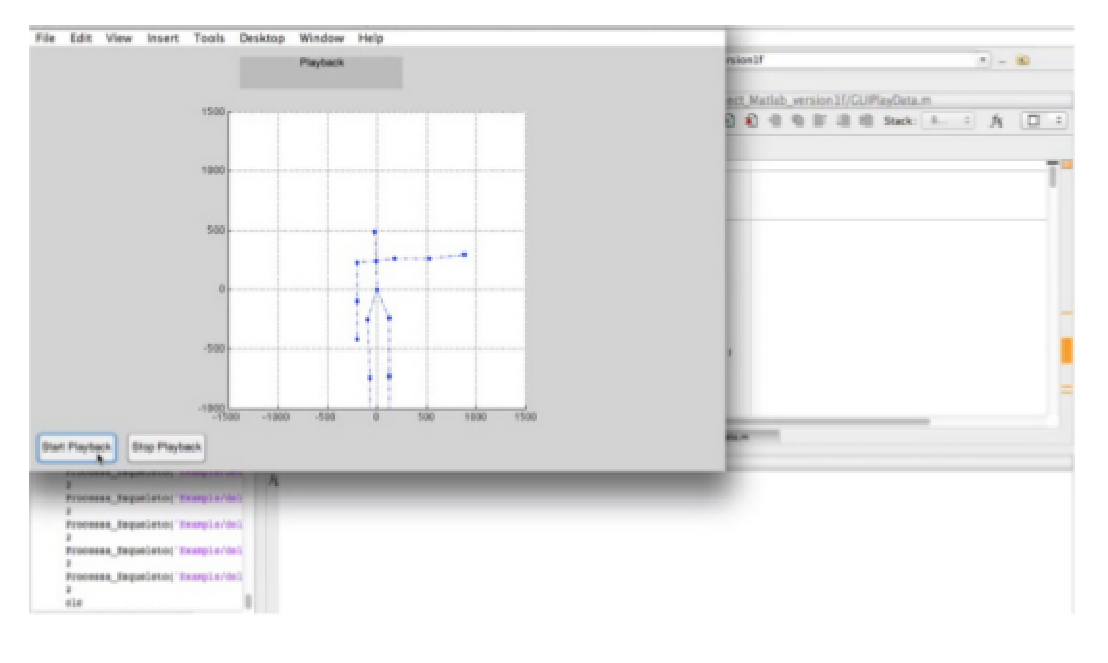
\includegraphics [keepaspectratio=true,scale=0.60]{figuras/movimentoReproducao.eps}

\caption{Reprodução do movimento. Fonte: \cite{roberto}.}

\label{movimentoReproducao}
\end{figure}

\begin{figure}[H]
\centering
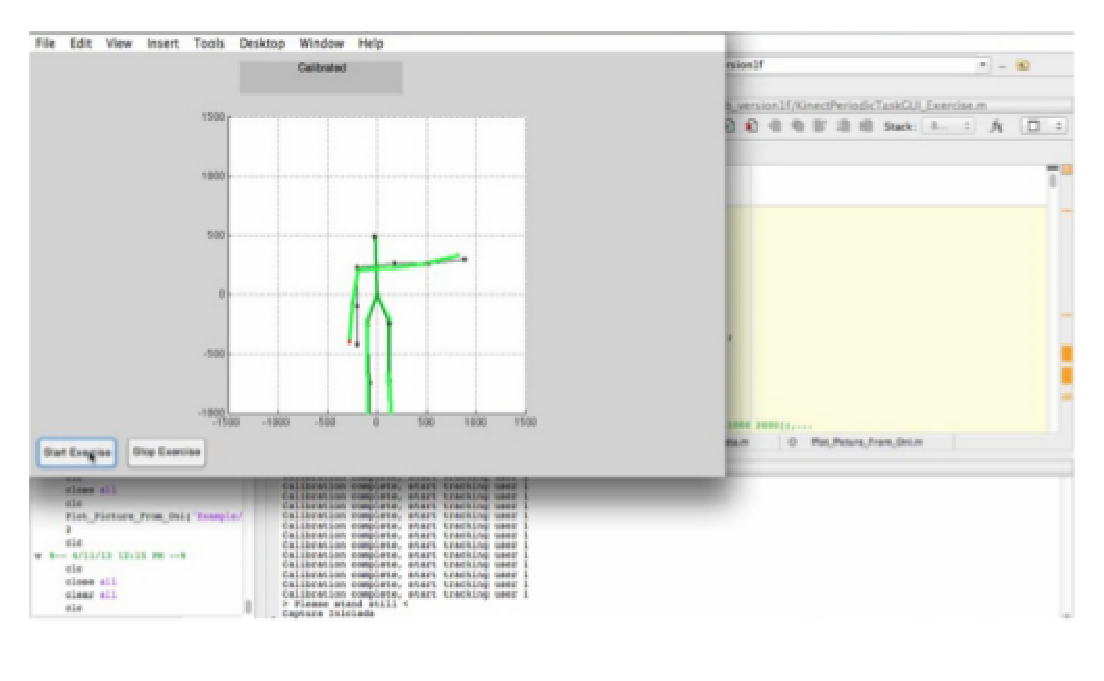
\includegraphics [keepaspectratio=true,scale=0.60]{figuras/movimentoCorreto.eps}

\caption{Movimento Correto. Fonte: \cite{roberto}.}
\label{movimentoCorreto}
\end{figure}

\begin{figure}[H]
\centering
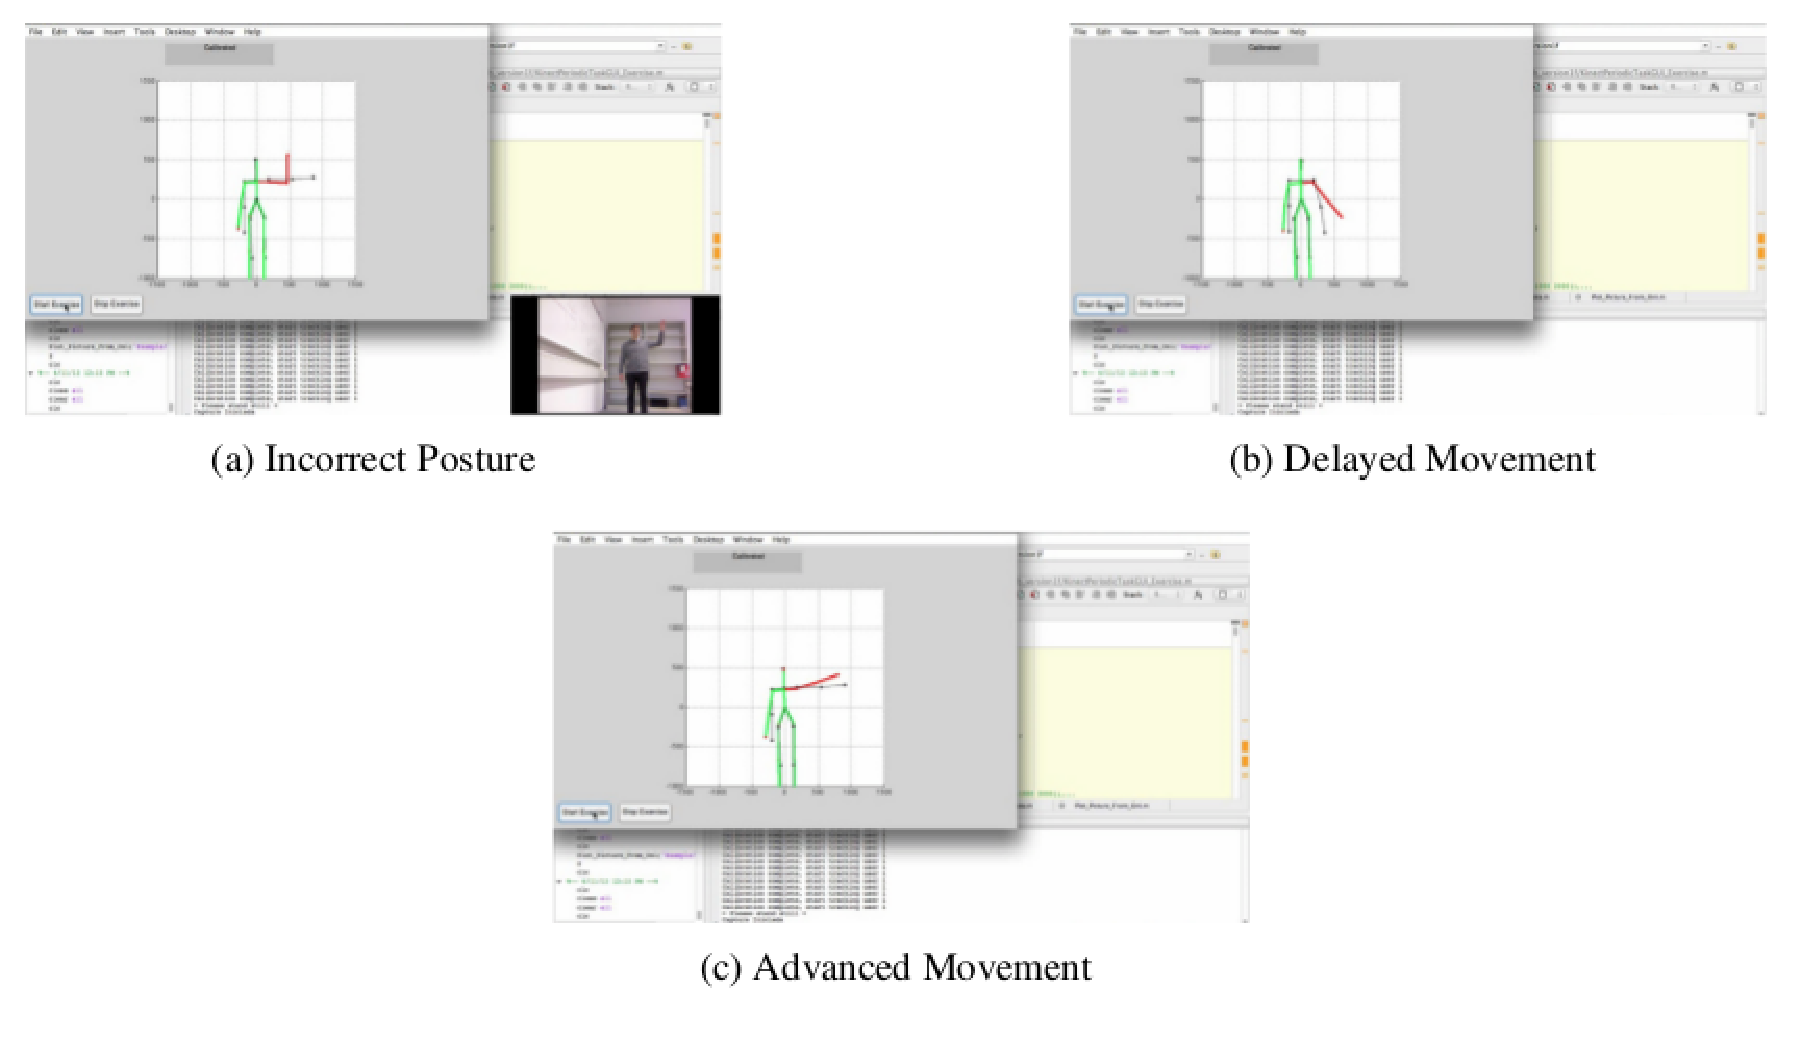
\includegraphics [keepaspectratio=true,scale=0.60]{figuras/movimentoIncorreto.eps}

\caption{Movimento Incorreto. Fonte: \cite{roberto}.}
\label{movimentoIncorreto}
\end{figure}

\section{Engenharia de Software}\label{sec:engenhariaSoft}
  Para o desenvolvimento de qualquer produto, necessita-se de um processo,
planejamento e projeto do produto. Para isso algumas técnicas e metodologias de
engenharia de software  aprendidas e utilizadas durante o curso, serão empregadas em
auxílio do desenvolvimento deste trabalho.
\subsection{Manifesto Ágil}
\label{sec:Manifesto Ágil}
  Afim de utilizar melhores maneiras para o desenvovlimento deste trabalho, foram utilizados alguns valores ágeis, onde podem ser encontrados
  no manifesto ágil. O manifesto ágil foi criado em 2001 e descreve um conjunto de abordagens para
desenvolvimento de software. Seus principais valores são:
  \begin{itemize}
  \item Indivíduos e interações a processos e ferramentas;
  \item Software funcionando a documentação compreensiva;
  \item Colaboração do cliente a negociação por contrato;
  \item Responder a mudanças a seguir um plano \cite{manifestoAgil}.
  \end{itemize}


\subsection{\textit{Kanban}}
\label{sec:kanban}
O \textit{Kanban} é uma metodologia popular usada por equipes que praticam o desenvolvimento ágil de software. Ele é extremamente proeminente entre as equipes de software ágil de hoje, mas sua metodologia de trabalho remonta a mais de 50 anos.

No fim dos anos 1940, a Toyota começou a otimizar seus processos de engenharia com base no mesmo modelo que os supermercados usavam para abastecer suas prateleiras. Os supermercados abastecem apenas a quantidade de produtos suficiente para atender à demanda dos consumidores, uma prática que otimiza o fluxo entre o supermercado e o consumidor.

Com o \textit{kanban}, as equipes de desenvolvimento ágil de software são capazes de aproveitar os princípios do JIT - \textit{just in time}, combinando a quantia do trabalho em andamento com a capacidade da equipe \cite{kanban1}.

O \textit{Kanban} eletrônico (\textit{e-Kanban}) é utilizado em substituição ao método físico, evitando alguns problemas como a perda de cartões e proporcionando mais rapidez na atualização do quadro de tarefas \cite{kanban}.



\subsection{Extreme programing - XP}
\label{sec:xp}
Extreme Programming (XP) é uma metodologia ágil de desenvolvimento de software,
nascida nos Estados Unidos ao final da década de 90. Tais objetivos são
alcançados através de um pequeno conjunto de valores, princípios
 e práticas, que também são baseados no manifesto ágil. Dentre seus princípios
e práticas, serão utilizados neste trabalho:

  \begin{itemize}
  \item Reuniões frequentes com os stakeholders (orientador).
  \item Design Incremental: O objetivo é criar a solução mais simples possível
  que seja suficiente para implementar as funcionalidades de cada iteração \cite{praticaXp}.
  \item Versionamento de código \cite{praticaXp}.
  \end{itemize}

  \section{Aquisição de dados com Sensores}
  \label{sec:aquisicaoSensores}

    Sensor pode ser entendido como dispositivo eletrônico que é sensível a determinada
  condição do ambiente, desde luminosidade, temperatura até a aceleração própria.
  No sistema desenvolvido junto a este trabalho é usado o kinect (\ref{sub:kinect}).


  \section{Processamento de sinais}
  \label{sec:processamentoSinais}
  Processamento de sinais consiste na análise e/ou modificação de sinais
(sequências discretas de números) de forma a extrair
informações dos mesmos e/ou torná-los mais apropriados para alguma aplicação específica \cite{processamentoSinais}.

   \section{Articulações no corpo humano}
   \label{sec:Juntas no corpo humano}
    A posição anatômica é uma posição de referência, que dá significado aos termos
    direcionais utilizados na descrição das partes e regiões do corpo. As discussões
    sobre o corpo, o modo como se movimenta, sua postura ou a relação entre uma e
   outra área assumem que o corpo como um todo está numa posição específica chamada
    posição anatômica.

     A tabela \ref{Juntas no corpo} mostra a articulação, seus movimentos e sua capacidade máxima em
   graus de movimentações.

   \begin{table}[H]
   \centering
   \caption{Articulações no corpo. Fonte: \cite{manualGoniometria}.}
   \label{Juntas no corpo}
   \begin{tabular}{|c|c|c|}
   \hline
   \rowcolor[HTML]{C0C0C0}
   Articulação                 & Movimento       & Grau de  Movimento \\ \hline
                               & Flexão          & 0-180              \\ \cline{2-3}
                               & Extensão        & 0-45               \\ \cline{2-3}
                               & Adução          & 0-40               \\ \cline{2-3}
                               & Abdução         & 0-180              \\ \cline{2-3}
                               & Rotação medial  & 0-90               \\ \cline{2-3}
   \multirow{-6}{*}{Ombro}     & Rotação lateral & 0-90               \\ \hline
                               & Flexão          & 0-145              \\ \cline{2-3}
   \multirow{-2}{*}{Cotovelo}  & Extensão        & 145-0              \\ \hline
                               & Pronação        & 0-90               \\ \cline{2-3}
   \multirow{-2}{*}{Radiulnar} & Supinação       & 0-90               \\ \hline
                               & Flexão          & 0-90               \\ \cline{2-3}
                               & Extensão        & 0-70               \\ \cline{2-3}
                               & Adução          & 0-45               \\ \cline{2-3}
   \multirow{-4}{*}{Punho}     & Abdução         & 0-20               \\ \hline
                               & Flexão          & 0-125               \\ \cline{2-3}
                               & Extensão        & 0-10               \\ \cline{2-3}
                               & Adução          & 0-15               \\ \cline{2-3}
\multirow{-4}{*}{Quadril}      & Abdução         & 0-45               \\ \hline
Joelho  & Flexão        & 0-140              \\ \hline
                            & Flexão dorsal         & 0-20               \\ \cline{2-3}
                            & Flexão plantar        & 0-40               \\ \cline{2-3}
                            & Adução          & 0-40               \\ \cline{2-3}
\multirow{-4}{*}{Tornozelo}     & Abdução         & 0-20               \\ \hline

   \end{tabular}
   \end{table}


  \subsection{Articulações no Unity 3D}
  \label{sec:Articulacoes no Unity 3D}
    Também chamadas de character joint elas são usadas para o chamado efeito
  boneco de pano (\textit{ragdoll effects}). A posição inicial de Referência é a
  a posição em T (\textit{T pose}). O unity não limita a angulação da articulação,
  deixando isso na mão do desenvolvedor, porém eles orientam ângulos máximos
  para estabilizar melhor seu avatar 3D \cite{unity3DManual}.

  \section{Restrição - \textit{Streaming}}
  \label{sec:restrição}
    Todo o processo, desde a aquisição do movimento ao processamento do sinal e a
  resposta para o usuário, deve ser em \textit{streaming}, para que o usuário possa corrijir a movimentação e se
  aproximar da correta execução do movimento. Para isso, temos que levar em conta
  a frequência de aquisição do sensor usado, o tempo do processamento de sinal e
  a frequência de atualização do monitor.

    O sensor kinect \cite{microsoftResearch}, tem uma frequência de
  aquisição de quadros de 30Hz, junto a um monitor com taxa de atualização de imagem
  para o usuário a 30Hz, assim a aproximadamente 33 milisegundos o
  sistema recebe um input do sensor e tem que em seguida apresentar um output. Isso restringe o processamento do sinal a 33 milissegundos de um input a outro, e
  também no tempo de atualização da imagem exibida para que não haja perda na
  fluidez e nem atraso na correção. As possíveis soluções para processamento de sinal nesse contexto serão apresentados nas seções seguintes.

  \subsection{Sistema distribuído}\label{distribuirProcessamento}
  Um sistema distribuído, sistema de processamento distribuído ou paralelo, é um sistema que interliga vários nós de processamento (computadores individuais) de maneira que um processo de grande consumo seja executado no nó mais disponível, ou mesmo subdividido por vários nós. Assim um sistema de processamento distribuído é uma "coleção de computadores independentes entre si que se apresenta ao usuário como um sistema único e coerente" \cite{tanenbaum}. A nomenclatura geralmente utilizada neste contexto é \textit{HPC (High Performance Computing)} e/ou \textit{DPC (Distributed/Parallel Computing)}.

  \subsection{Sistema multiprocessado}\label{multiprocessamento}
  Um multiprocessador ou sistema multiprocessado é um sistema integrado de computação com as seguintes características:
\begin{itemize}
  \item Envolve dois ou mais processadores físicos (sejam processadores separados ou múltiplos núcleos encapsulados no mesmo chip) ou lógicos
   (processador(es) com a tecnologia \textit{HyperThreading} da Intel) com o mesmo poder computacional e cada um capaz de executar processos autonomamente.
   Isto implica que não há nenhuma unidade central de controle, cada processador contém sua própria unidade de controle. Assim, efetivamente, a lógica de controle é distribuída pelo sistema.

  \item Os processadores compartilham um único espaço de endereçamento de memória.
  \item O sistema de hardware é como um todo gerenciado por um único sistema operacional.
\end{itemize}

  O sistema operacional com suporte a multiprocessamento deve ser capaz de:
  \begin{itemize}
    \item Suportar multitarefa;
    \item Manter múltiplas filas de processos, uma para cada processador \cite{os}.

  \end{itemize}

  \subsection{Processamento massivamente paralelo}\label{massivamenteParalelo}
  MPP (\textit{Massively Parallel processing} - Processamento Massivamente Paralelo), é o processamento coordenado
  de um programa por vários processadores que funcionam em diferentes partes do programa,
   com cada processador usando seu próprio sistema operacional e memória.
    Normalmente, os processadores MPP se comunicam usando alguma interface de mensagens.

     Em algumas implementações, até 200 ou mais processadores podem funcionar no mesmo aplicativo.
      Um arranjo de "interconexões" de caminhos de dados permitem que mensagens sejam enviadas entre os processadores.
       Normalmente, a configuração para MPP é mais complicada, exigindo pensar sobre como particionar um banco de dados
        comum entre processadores e como atribuir trabalho entre eles.
         Um sistema MPP também é conhecido como um sistema "vagamente acoplado" ou "nada compartilhado" \cite{mpp}.

  \section{Trabalho relacionado}
  \label{Sec:MetCondTCC}
    O desenvolvimento deste trabalho foi inspirado no algoritmo do Roberto de Souza Baptista \cite{roberto}.
  e podemos afirmar que ele pertence a área da engenharia biomédica. "Classicamente,
  a Engenharia Biomédica é vista como a aplicação dos métodos de distintas áreas
  das Ciências Exatas e de Engenharia no campo das Ciências Médicas e
  Biológicas" \cite{engenhariaBiomedica}. Ele desenvolve uma abordagem
  inovadora aplicado a terapia de  doenças/acidentes motores, aplicado a
   fiosioterapia. Onde desenvolve uma nova abordagem para análise de movimentos.

  \subsection{Protótipo}
  \label{Sec:protótipo}
    Junto com o algoritmo citado anteriormente \cite{roberto}, foi
  desenvolvido um protótipo no software matlab \cite{matlab}. Esse sistema inicial
  implementou algumas das teorias do exame. Ele possui três etapas: rotular os dados,
  parametrização e utilizar para segmentação automática.
  \begin{itemize}

  \begin{sloppypar}

  \item \textbf{Rotulação}: Na etapa de rotular os dados,começando pelo arquivo
  ' SCRIPT\_labelAndIndexMultivariateFile\_WBM21.m '. Neste script estão duas funções,
  \textit{labelAndIndexUnivariateFile} que por sua vez chama a função
  \textit{labelAndIndexUnivariateStructDataset} que chama a função \textit{labelAndIndexUnivariateDataset}
  e \textit{transitionIndexMultivariateFile}.Os dados de entrada são puxados dos arquivos da pasta
  'PreProcessedData','/',DecRateN\_Filter,'/',Movement,'/',Subject,'/',Trial,'.mat'.
  Esses dados foram coletados previamente por sensores. Os dados são uma struct .mat
  com  os ângulos de algumas articulações e o tempo. Esses ângulos são dados em radianos
   e são divididos em articulações e em uma única coluna como podemos observar em \ref{structMatlab}.

  \begin{figure}[!h]
  \centering
  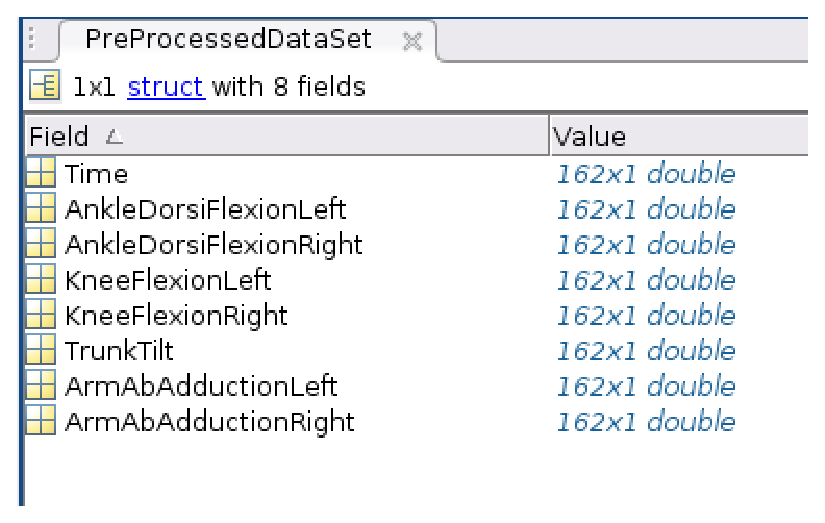
\includegraphics [keepaspectratio=true,scale=0.60]{figuras/structMatlab.eps}
  \caption{Dados das articulações}
  \label{structMatlab}
  \end{figure}

    Quando o script é executado  primeiro um gráfico é traçado com várias curvas
   para selecionar o início e fim de cada conjunto de dados,
  depois cada curva é apresentada separadamente. Essa é a etapa para rotular os
  dados de cada curva. No prompt ele pergunta qual o “\textit{Switch Variable}”, em seguida
   ele pede para marcar  o início e o fim do intervalo com esse rótulo. A seguir
  pergunta se é o fim do  conjunto de dados. Caso não seja o fim ele volta a
   perguntar qual a “Switch Variable”. Esse procedimento se repete para todas as curvas.
  Logo após, vem a parte que rotula os dados multivariáveis dependendo do conjunto
  de rótulos de cada variável separada. O resultado é a struct “thisLabeledIndexStructDataSet” salvo na pasta
  LabeledDataMultivariate’/‘,DecRateN\_Filter,'/',Movement,'/',Subject,'/',Trial,'.mat'.

  \item \textbf{Parametrização}: Na etapa de parametrização do modelo a função:
   \"SLDS\_Univariate\_ParameterDataSetBuilder2.m\" pega os dados rotulados da etapa
  anterior, ou seja os dados segmentados automaticamente e com as funções
  “parametersCteVelSpaceStateModel2” e “hmmTransitionMatrix2” calcula os parâmetros
  do Modelo Oculto de Markov. Esta função é a base para o script
  "SLDS\_Univariate\_IntraSubject\_ParameterDataset\_Script.m”  que pega diversos
   conjuntos de dados rotulados, de diferentes sujeitos ou diferentes execuções
  do mesmo sujeito e chama a função “SLDS\_Univariate\_ParameterDataSetBuilder2.m”
   para cada um deles e no fim temos os parâmetros do modelo oculto de Markov ajustado
   para vários conjuntos de treinamento.

  \end{sloppypar}
  \item \textbf{Segmentação}: Esse é o programa que faz a estimação dos rótulos associado com cada medida.
  A principal função é a “SLDS\_Filter\_Univariate” ela recebe as structs
  ValidationTrialThisVariable e FittedModelThisVariable e a variável
  InitialSwitchVariableState. A ValidationTrialThisVariable contém os dados a serem
   classificados e pode conter também os rótulos. São as medidas do movimento, os
  mesmos dados usados na parte de rotulação. O FittedModelThisVariable são todos
  os parâmetros do modelo (análogo aos parâmetros do ModeloOculto de Markov).
  A variável InitialSwitchVariableState indica o símbolo da primeira medida.

  Na imagem \ref{diagramProt} podemos ver todo o fluxo de dados do protótipo.
  \end{itemize}

  \begin{figure}[H]
  \centering
  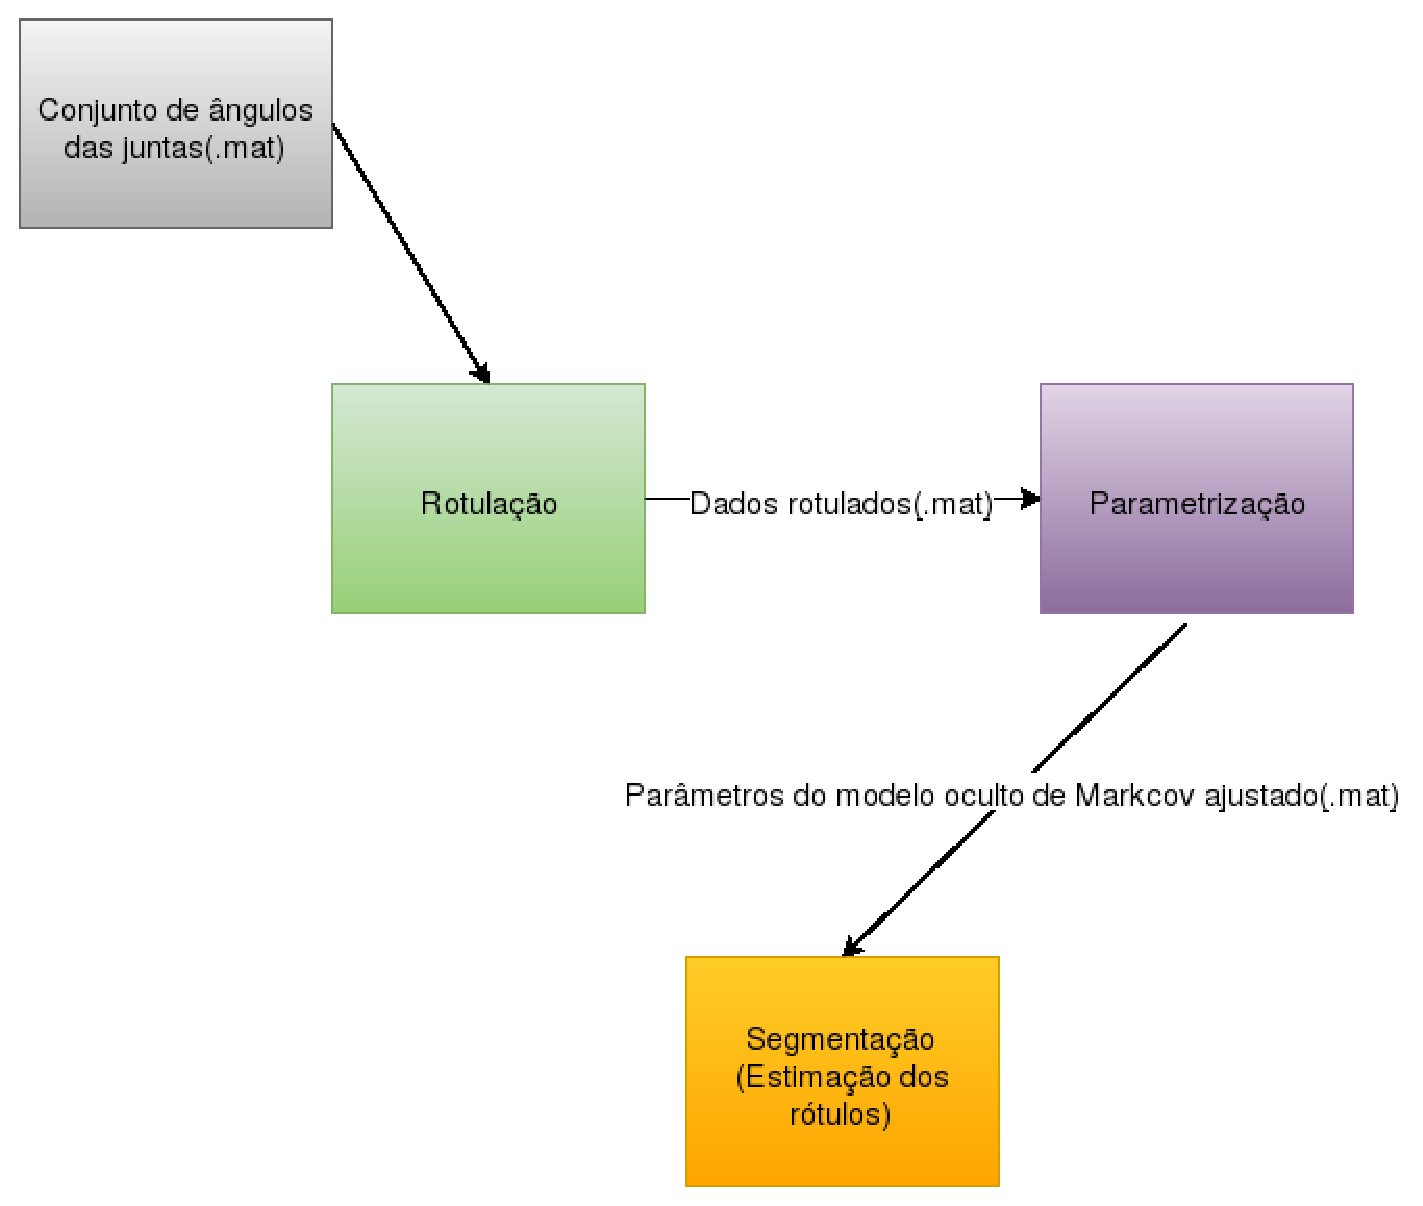
\includegraphics [keepaspectratio=true,scale=0.60]{figuras/diagramProt.eps}
  \caption{Fluxo de Dados}
  \label{diagramProt}

  \end{figure}


  \section {Requisitos}
  \label{Sec:Requisitos}
    Um requisito é definido como "uma condição ou uma capacidade com a qual o
  sistema deve estar de acordo". Existem vários tipos de
  requisitos. Um modo de categorizá-los é descrito como o modelo
  FURPS+ \cite{robertGrady}.

  FURPS+ é um sistema para a classificação de requisitos, o acrônimo representa categorias que podem ser usadas na definição de requisitos, assim como representa atributos de Qualidade de Software, sendo ele parte do Rational Unified Process (RUP):
\begin{itemize}

\item Functionality (Funcionalidade) – Representa todo aspecto funcional do software, seus requisitos. É uma categoria com diversas subcategorias que variam de acordo com a aplicação. Sua medição considera, principalmente, o cumprimento dos requesitos especificados.

\item Usability (Usabilidade) – É o atributo que avalia a interface com o usuário. Possui diversas subcategorias, entre elas: prevenção de erros; estética e design; ajudas (Help) e documentação; consistência e padrões.

\item Reliability (Confiabilidade) – Refere-se a integridade, conformidade e interoperabilidade do software. Os requisitos a serem considerados são: freqüência e gravidade de falha; possibilidade de recuperação; possibilidade de previsão; exatidão; tempo médio entre falhas (MTBF).

\item Performance (Desempenho) – Avalia os requisitos de desempenho do software. Podendo usar como medida diversos aspectos, entre eles: tempo de resposta, consumo de memória, utilização da CPU, capacidade de carga e disponibilidade da aplicação.

\item Supportability (Suportabilidade) – os requisitos de suportabilidade agrupam várias características, como: testabilidade, adaptabilidade, manutenibilidade, compatibilidade, configurabilidade, instalabilidade, escalabilidade, localizabilidade entre outros.
\end{itemize}
O “+” do acrônimo engloba outros requisitos não-funcionais que devem ser lembrados:
\begin{itemize}
\item Requisitos de design (desenho) – Um requisito de design, freqüentemente chamado de uma restrição de design, especifica ou restringe o design de um sistema. Exemplos podem incluir: linguagens de programação, processo de software, uso de ferramentas de desenvolvimento, biblioteca de classes, etc.
\item Requisitos de implementação – Um requisito de implementação especifica ou restringe o código ou a construção de um sistema. Como exemplos, podemos citar:
\begin{itemize}

  \item padrões obrigatórios;
  \item linguagens de implementação;
  \item políticas de integridade de banco de dados;
  \item limites de recursos;
  \item ambientes operacionais.

\end{itemize}
\item Requisitos de interface – especifica ou restringe as funcionalidades inerentes a interface do sistema com usuário.
\item Requisitos físicos – especifica uma limitação física pelo hardware utilizado, por exemplo: material, forma, tamanho ou peso. Podendo representar requisitos de hardware, como as configurações físicas de rede obrigatórias \cite{rational}.
\end{itemize}

  \section{Arquitetura de software}
  \label{Sec:arquitetura}
    De acordo com a ISO/IEEE 1471-2000 - Arquitetura é a organização fundamental
  de um sistema incorporada em seus componentes, seus relacionamentos com o
  ambiente, e os princípios que conduzem seu design e evolução.

    A arquitetura de software, consiste na definição dos componentes de software,
     suas propriedades externas, e seus relacionamentos. A documentação da arquitetura do software
      facilita: a comunicação entre os \textit{stakeholders},
       e permite o reúso do projeto.
